%!TEX root = report.tex	
\begin{subfigure}{0.16\textwidth}
	\centering
	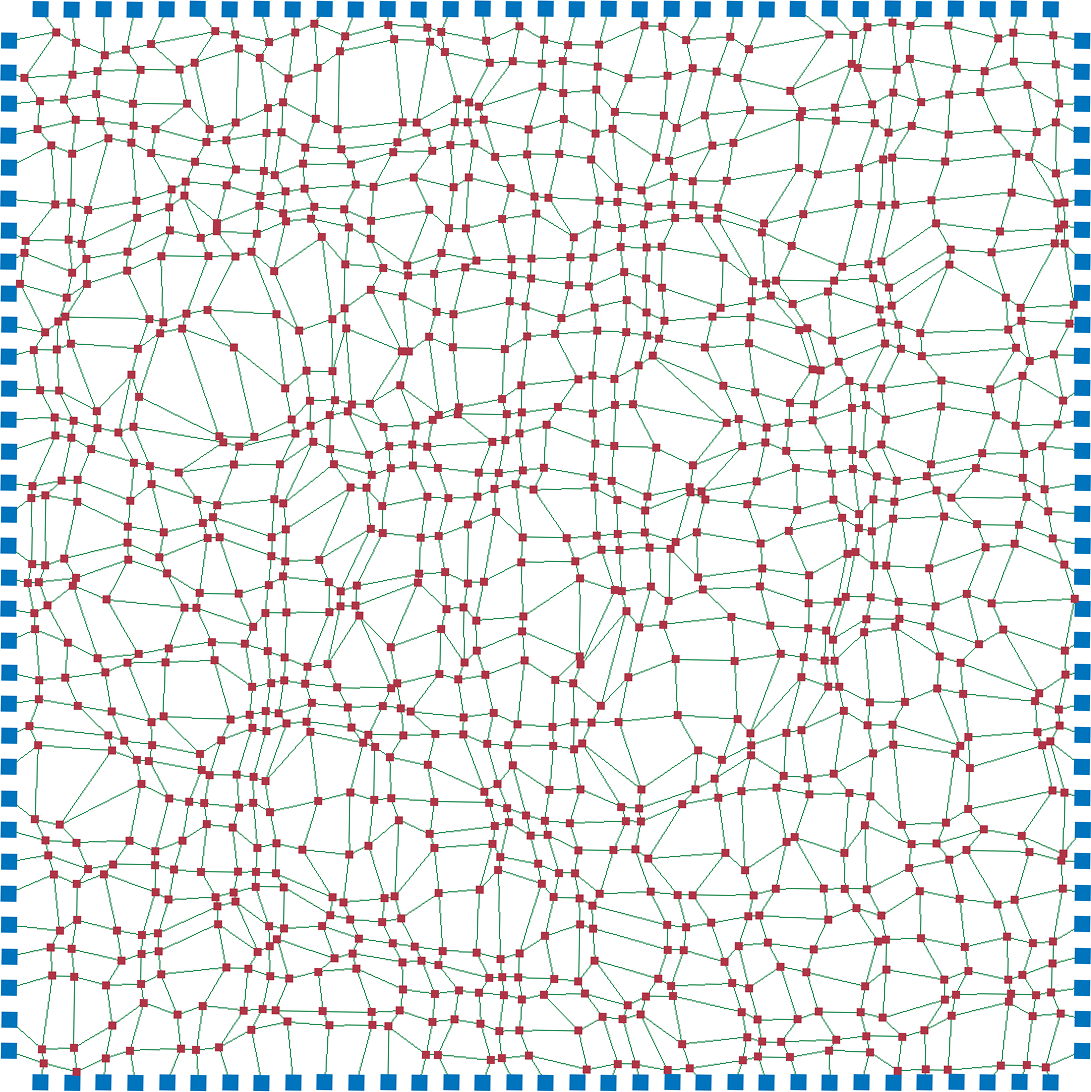
\includegraphics[
		width=\textwidth, 
		height=\textwidth, 
		keepaspectratio=true]
	{./img/results/1200_0_1_highest_97_step_0}
	\caption{}
	\label{fig:experiment:highestStrain:0}
\end{subfigure}
\begin{subfigure}{0.16\textwidth}
	\centering
	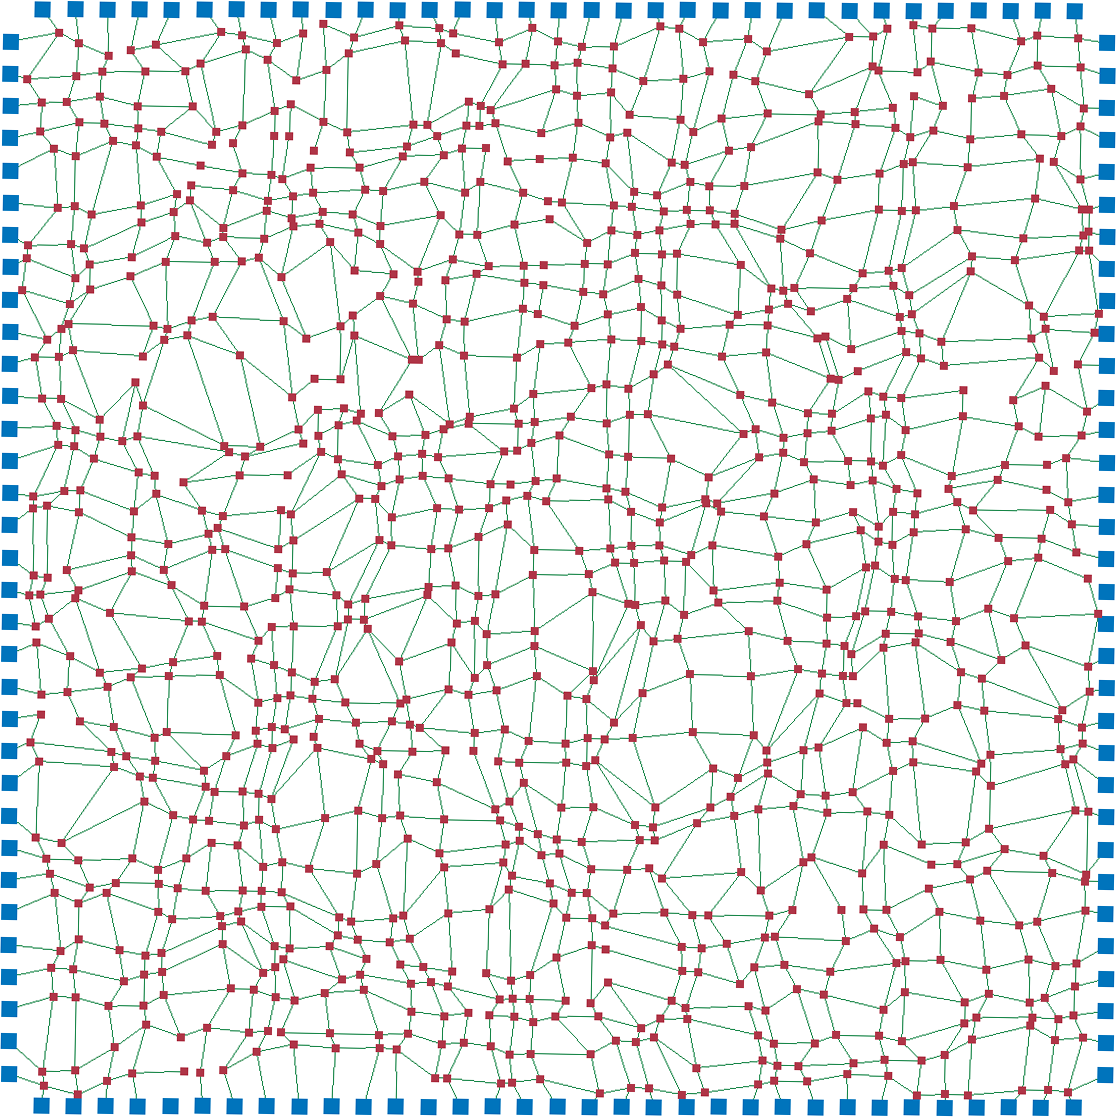
\includegraphics[
		width=\textwidth, 
		height=\textwidth, 
		keepaspectratio=true]
	{./img/results/1200_0_1_highest_97_step_1}
	\caption{}
	\label{fig:experiment:highestStrain:1}
\end{subfigure}	
\begin{subfigure}{0.16\textwidth}
	\centering
	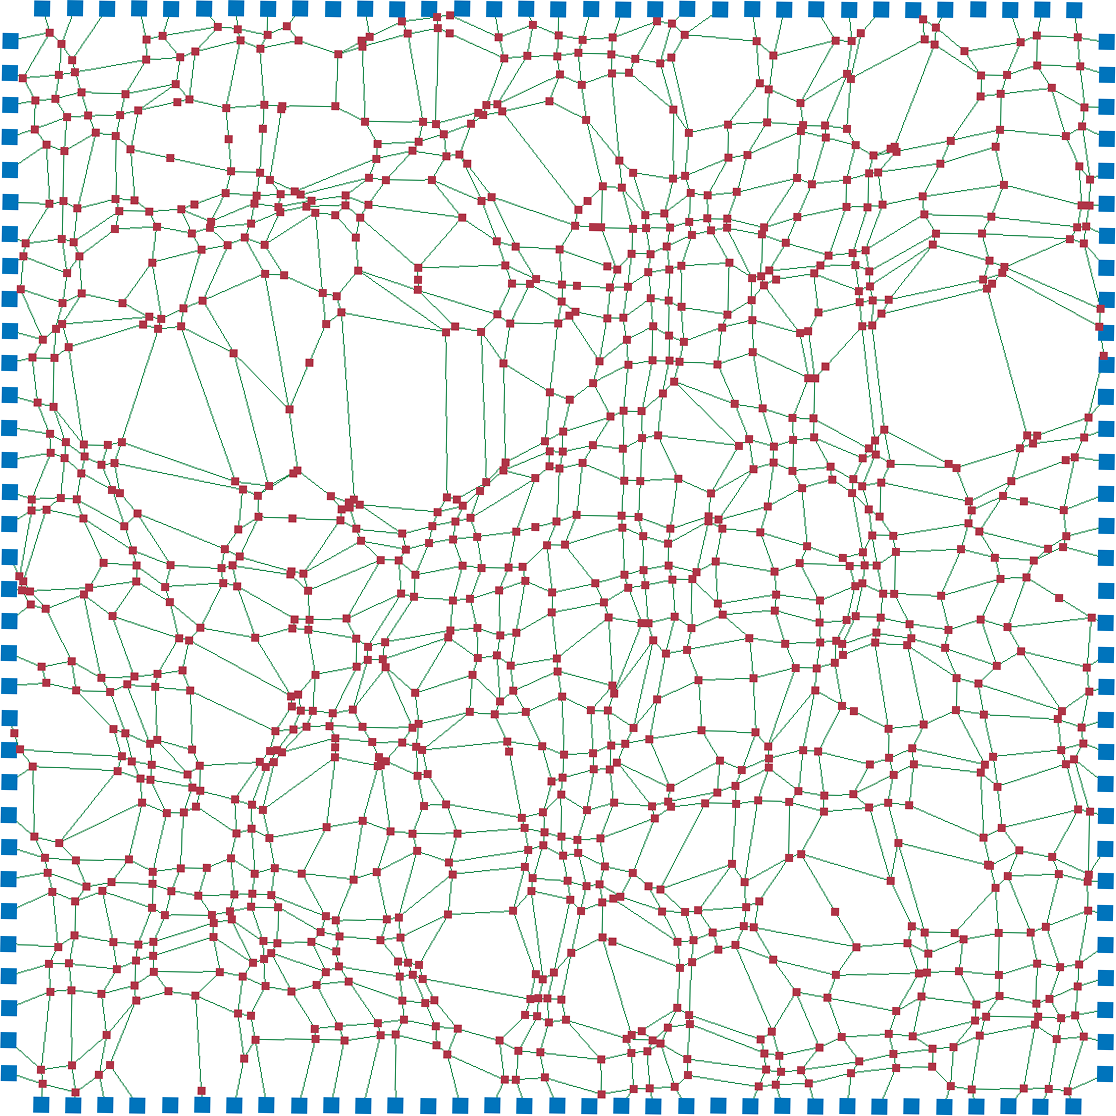
\includegraphics[
		width=\textwidth, 
		height=\textwidth, 
		keepaspectratio=true]
	{./img/results/1200_0_1_highest_97_step_2}
	\caption{}
	\label{fig:experiment:highestStrain:2}
\end{subfigure}		
\begin{subfigure}{0.16\textwidth}
	\centering
	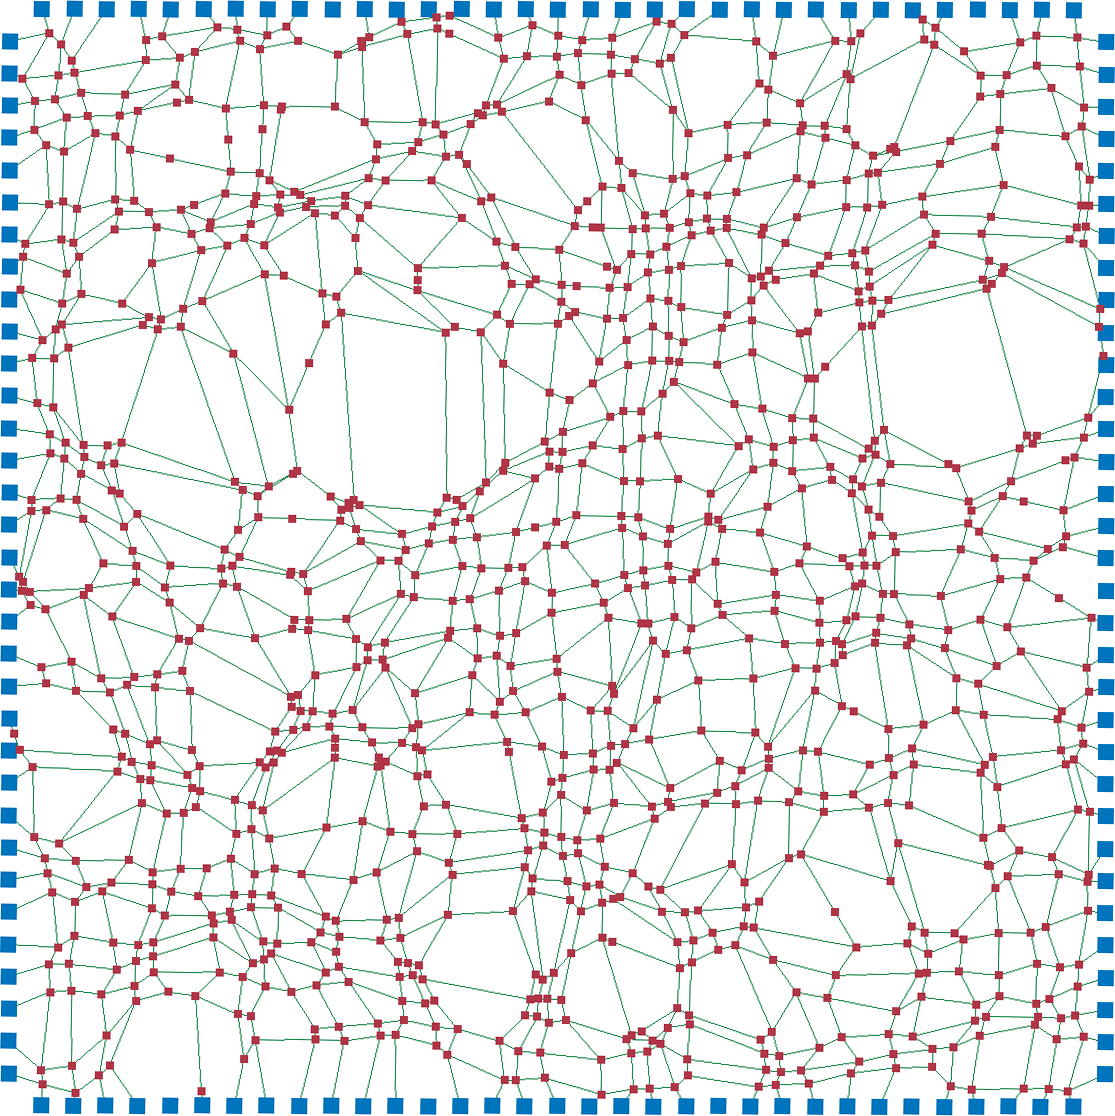
\includegraphics[
		width=\textwidth, 
		height=\textwidth, 
		keepaspectratio=true]
	{./img/results/1200_0_1_highest_97_step_3}
	\caption{}
	\label{fig:experiment:highestStrain:3}
\end{subfigure}			
\begin{subfigure}{0.16\textwidth}
	\centering
	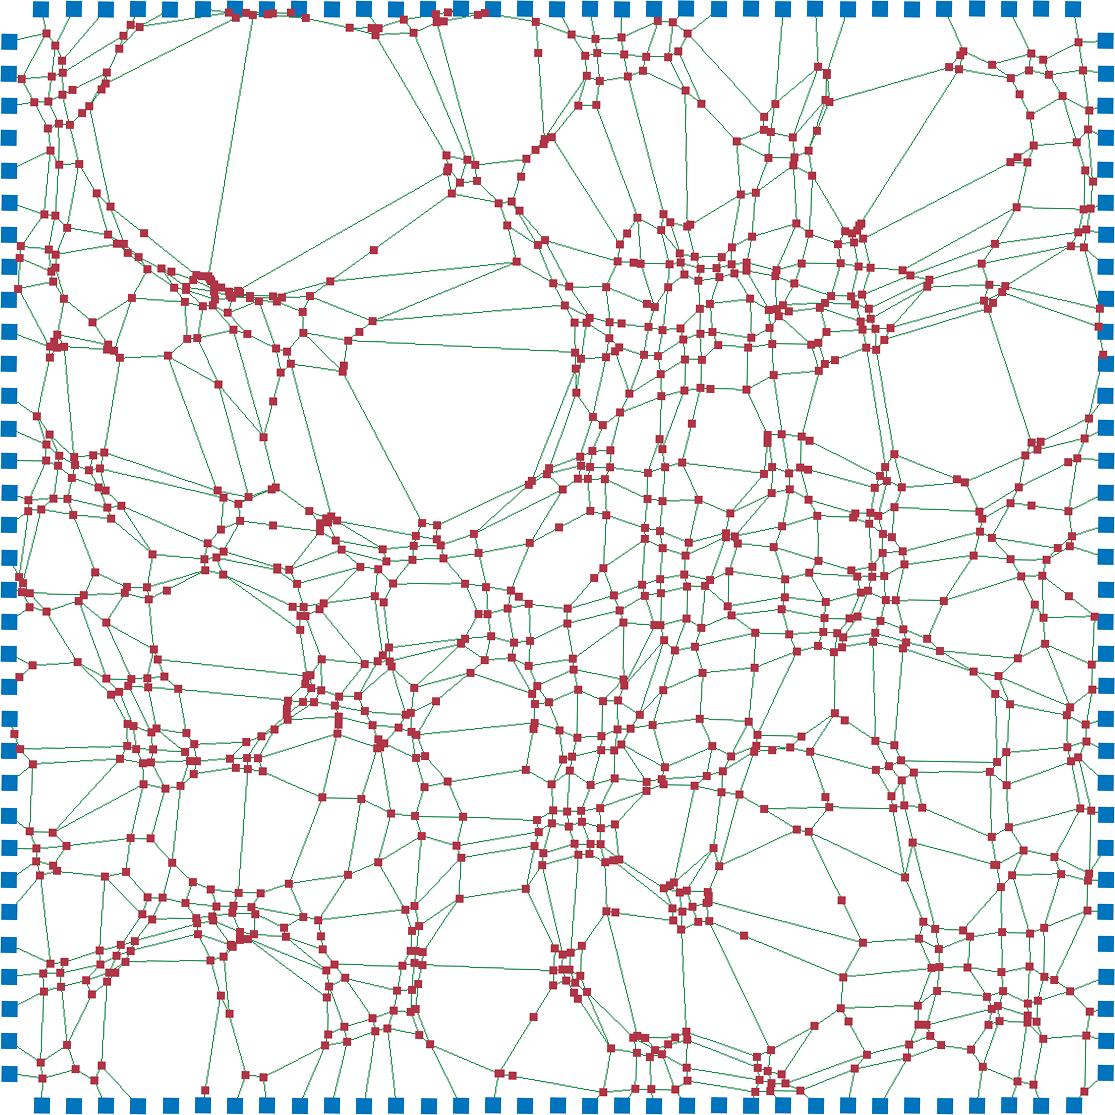
\includegraphics[
		width=\textwidth, 
		height=\textwidth, 
		keepaspectratio=true]
	{./img/results/1200_0_1_highest_97_step_4}
	\caption{}
	\label{fig:experiment:highestStrain:4}
\end{subfigure}				
\begin{subfigure}{0.16\textwidth}
	\centering
	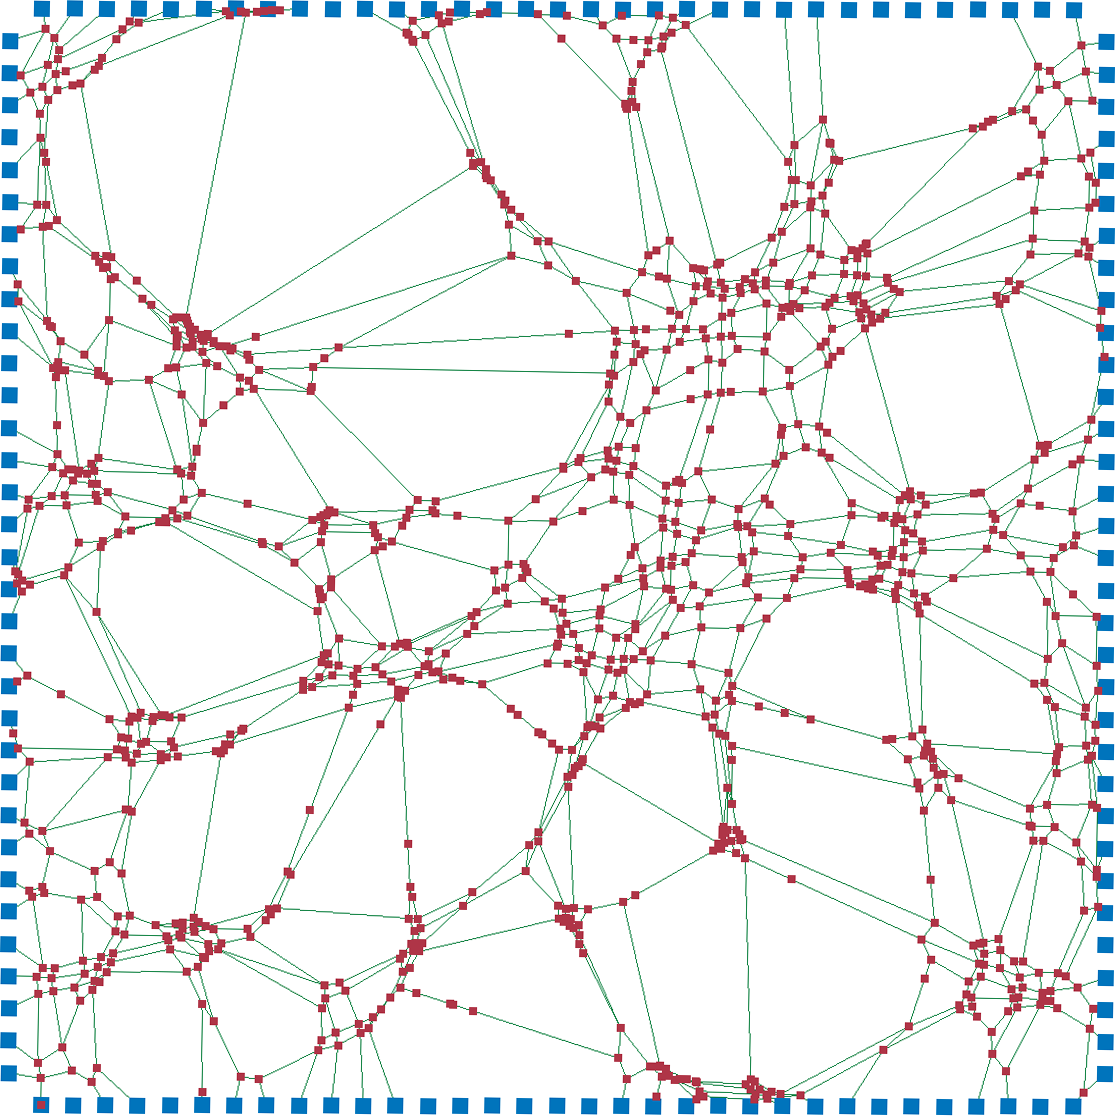
\includegraphics[
		width=\textwidth, 
		height=\textwidth, 
		keepaspectratio=true]
	{./img/results/1200_0_1_highest_97_step_5}
	\caption{}
	\label{fig:experiment:highestStrain:5}
\end{subfigure}
\begin{subfigure}{0.16\textwidth}
	\centering
	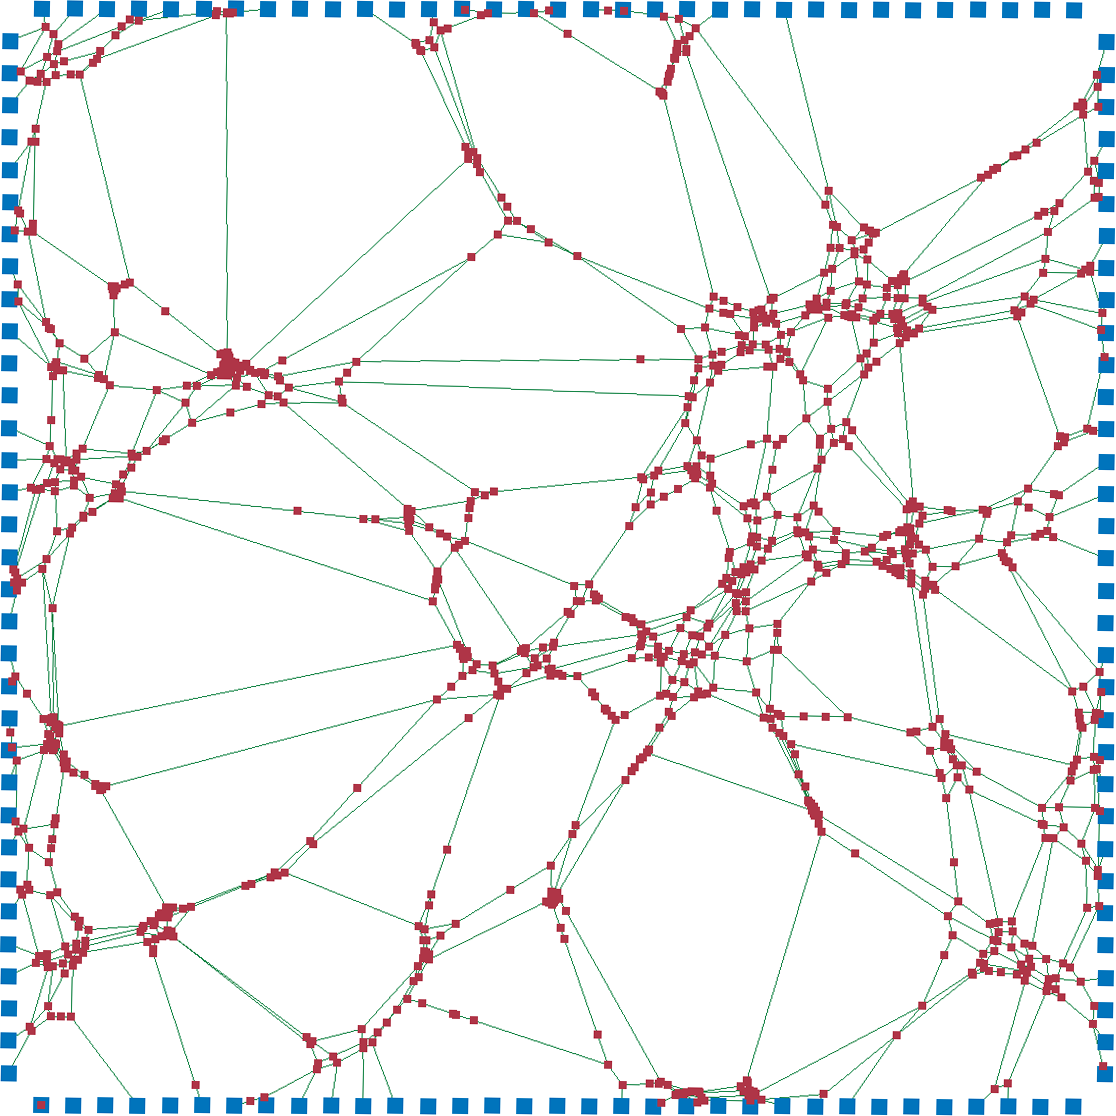
\includegraphics[
		width=\textwidth, 
		height=\textwidth, 
		keepaspectratio=true]
	{./img/results/1200_0_1_highest_97_step_6}
	\caption{}
	\label{fig:experiment:highestStrain:6}
\end{subfigure}	
\begin{subfigure}{0.16\textwidth}
	\centering
	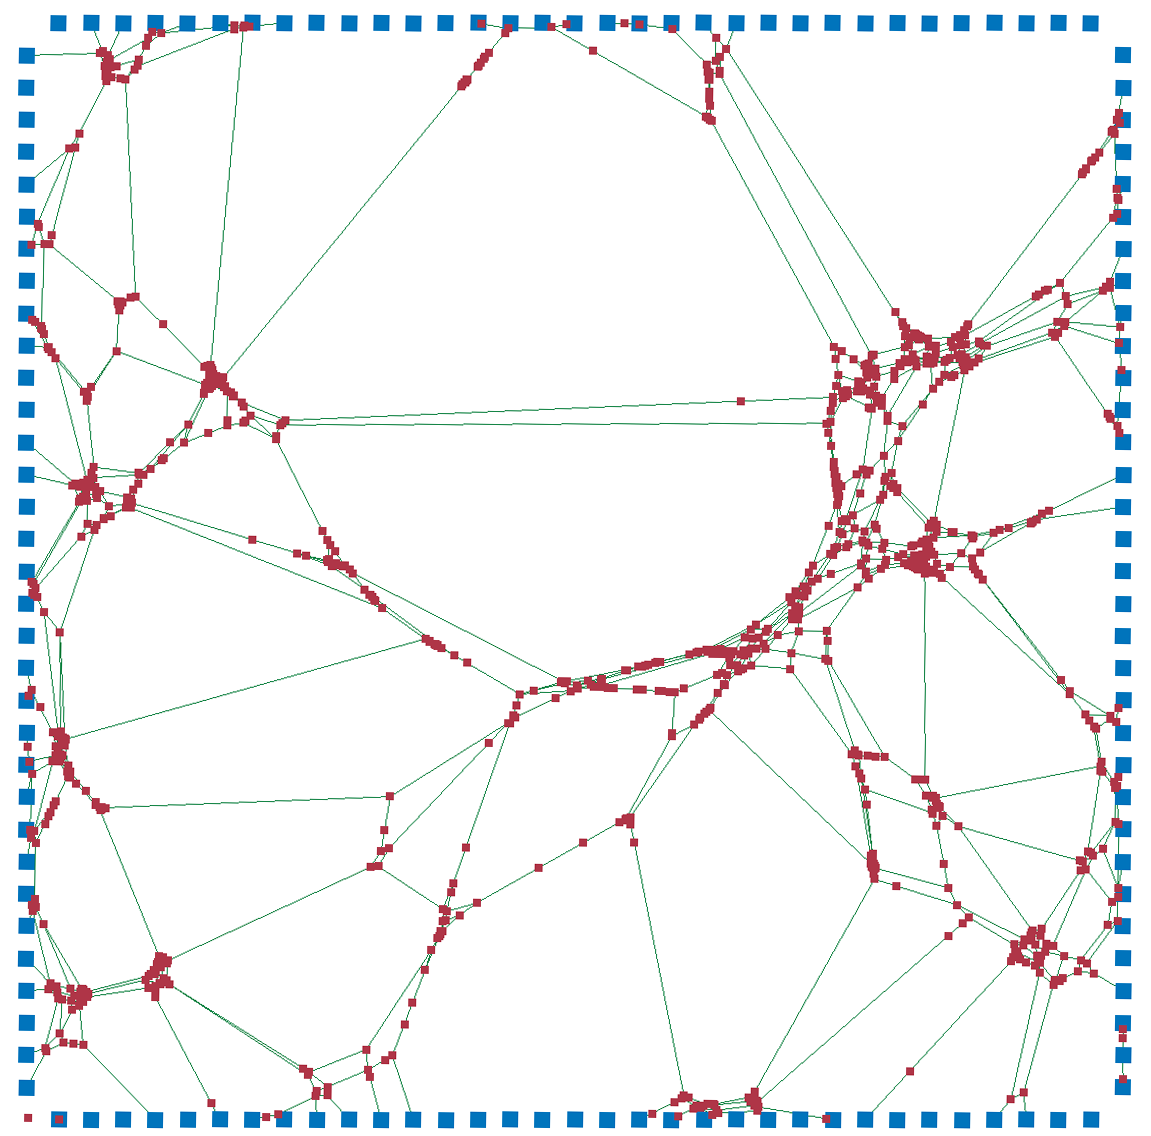
\includegraphics[
		width=\textwidth, 
		height=\textwidth, 
		keepaspectratio=true]
	{./img/results/1200_0_1_highest_97_step_7}
	\caption{}
	\label{fig:experiment:highestStrain:7}
\end{subfigure}		
\begin{subfigure}{0.16\textwidth}
	\centering
	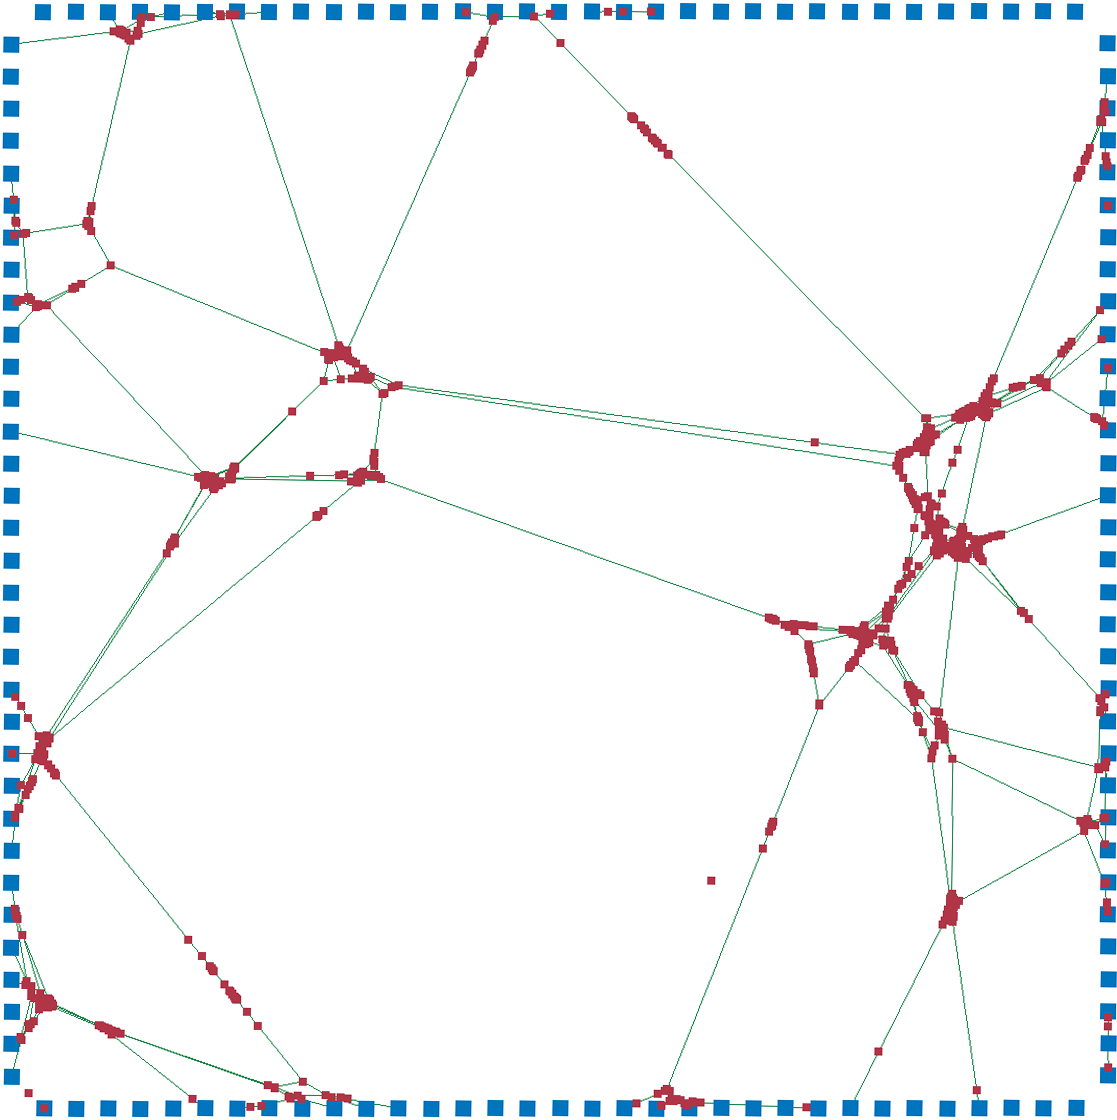
\includegraphics[
		width=\textwidth, 
		height=\textwidth, 
		keepaspectratio=true]
	{./img/results/1200_0_1_highest_97_step_8}
	\caption{}
	\label{fig:experiment:highestStrain:8}
\end{subfigure}			
\begin{subfigure}{0.16\textwidth}
	\centering
	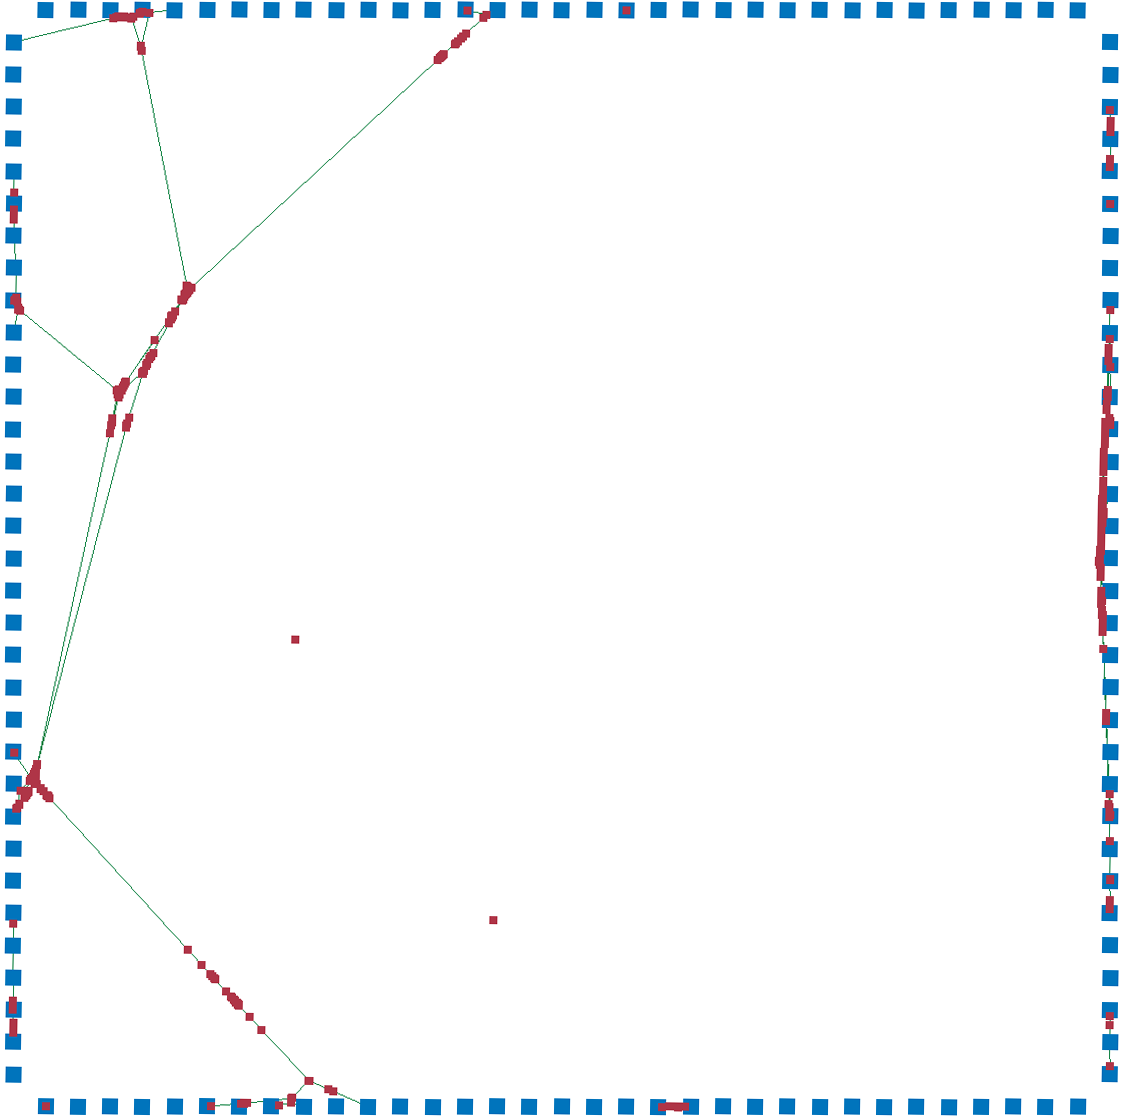
\includegraphics[
		width=\textwidth, 
		height=\textwidth, 
		keepaspectratio=true]
	{./img/results/1200_0_1_highest_97_step_9}
	\caption{}
	\label{fig:experiment:highestStrain:9}
\end{subfigure}					
\begin{subfigure}{0.16\textwidth}
	\centering
	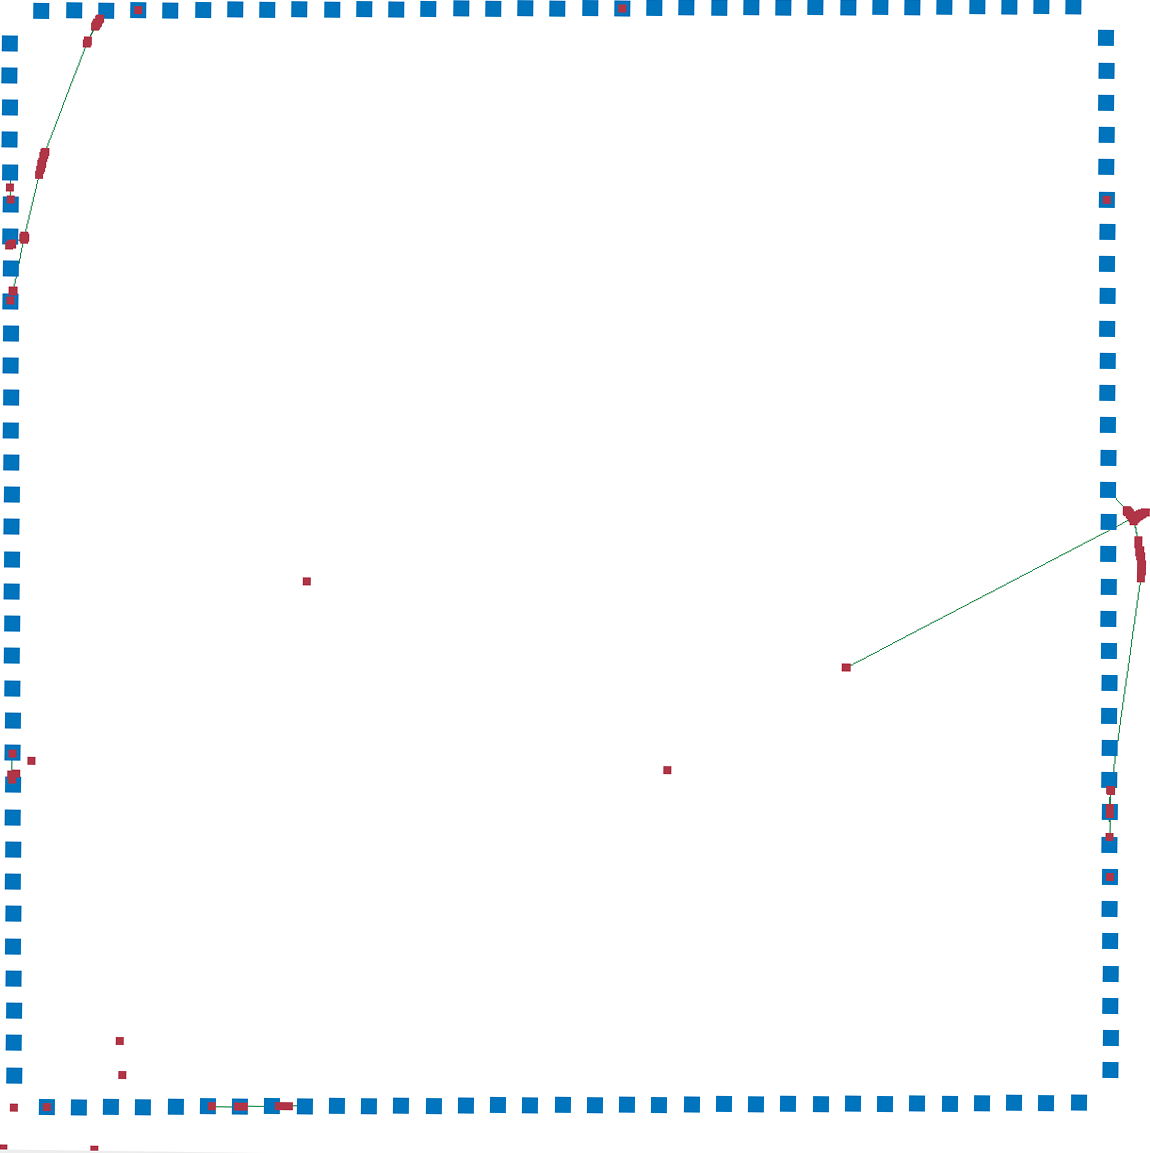
\includegraphics[
		width=\textwidth, 
		height=\textwidth, 
		keepaspectratio=true]
	{./img/results/1200_0_1_highest_97_step_10}
	\caption{}
	\label{fig:experiment:highestStrain:10}
\end{subfigure}			
\begin{subfigure}{0.16\textwidth}
	\centering
	
\includegraphics[
		width=\textwidth, 
		height=\textwidth, 
		keepaspectratio=true]
	{./img/results/1200_0_1_highest_97_step_11}
	\caption{}
	\label{fig:experiment:highestStrain:11}
\end{subfigure}	